\section[General arg]{General Options - source faults}

\graphicspath{{Chapter4/Figs/Vector/}{Figs/}}
% //////////////////////////////////////////////////////////////////////////////
\begin{frame}
  \frametitle{General Options - source faults}
  \framesubtitle{}
  \label{fr4:hist_pics}
\begin{scriptsize}
\begin{itemize}
\item
  \texttt{-r\ \ \ \textbar{}\ -\/-region}: set custom region parameters.
  \emph{Structure} \texttt{-r\ minlon\ maxlon\ minlat\ maxlat\ prjscale}
\item
  \texttt{-t\ \ \ \textbar{}\ -\/-topography}: plot topography using DEM
  file
\item
  \texttt{-o\ \ \textbar{}\ -\/-output\ \textless{}filename\textgreater{}}:
  set custom name of output file. Default is
  \texttt{\textless{}inputdata\textgreater{}}.
\item
  \texttt{-cmt\ \textbar{}\ -\/-moment\_tensor\ \textless{}file\textgreater{}}
  : Plot Centroid Moment Tensors list of earthquakes.
\item
  \texttt{-ed\ \textbar{}\ -\/-eq\_distribution\ \textless{}file\textgreater{}}
  : Plot earthquakes distribution. No classification.
\item
  \texttt{-fl\ \textbar{}\ -\/-faults\_db}: Plot custom fault database
  catalogue.
\item
  \texttt{-mt\ \textbar{}\ -\/-map\_title\ \ "map\ title"}: Custom map
  title.
\item
  \texttt{-ct\ \textbar{}\ -\/-custom\_text\ \ \textless{}path\ to\ file\textgreater{}}
  : Plot Custom text file.
\item
  \texttt{-lg\ \textbar{}\ -\/-logo\_gmt}: Plot GMT logo and time stamp.
\item
  \texttt{-lc\ \textbar{}\ -\/-logo\_custom}: Plot custom logo (image)
  of your organization.
\item
  \texttt{-h\ \textbar{}\ -\/-help}: Help menu.
\item
  \texttt{-v\ \textbar{}\ -\/-version}: Plot version.
\item
  \texttt{-d\ \textbar{}\ -\/-debug}: Enable Debug option.
\end{itemize}
\end{scriptsize}
\end{frame}
\note{}

% //////////////////////////////////////////////////////////////////////////////
\begin{frame}
  \frametitle{General Options - source faults}
  \framesubtitle{Plot fault parameters}
  \label{fr4:hist_pics}

\emph{Plot fault geometry}

\begin{scriptsize}
\begin{itemize}
\item
  \texttt{-fproj}: Plot source and receiver faults' trace at surface.
\item
  \texttt{-fsurf}: Plot surface of source and receiver faults.
\item
  \texttt{-fdep}: Plot intersection of target depth with fault plane.
\end{itemize}
\end{scriptsize}

\emph{Adjust and convert output format}
\begin{scriptsize}
\begin{itemize}
\item
  \texttt{-outjpg} : Adjust and convert to JPEG.
\item
  \texttt{-outpng} : Adjust and convert to PNG (transparent where
  nothing is plotted).
\item
  \texttt{-outeps} : Adjust and convert to EPS.
\item
  \texttt{-outpdf} : Adjust and convert to PDF.
\end{itemize}
\end{scriptsize}
\end{frame}
\note{}

% //////////////////////////////////////////////////////////////////////////////
\begin{frame}[t,fragile]
  \frametitle{General Options - source faults}
  \framesubtitle{Plot fault parameters}
  \label{fr4:hist_pics}
\begin{columns}[t]
  \begin{column}{.5\textwidth}
\begin{scriptsize}
\begin{verbatim}
$ ./coulomb2gmt.sh kef_1953 kef_1953_kef \
                   -outjpg -o example401 \
\end{verbatim}
\end{scriptsize}
\centering
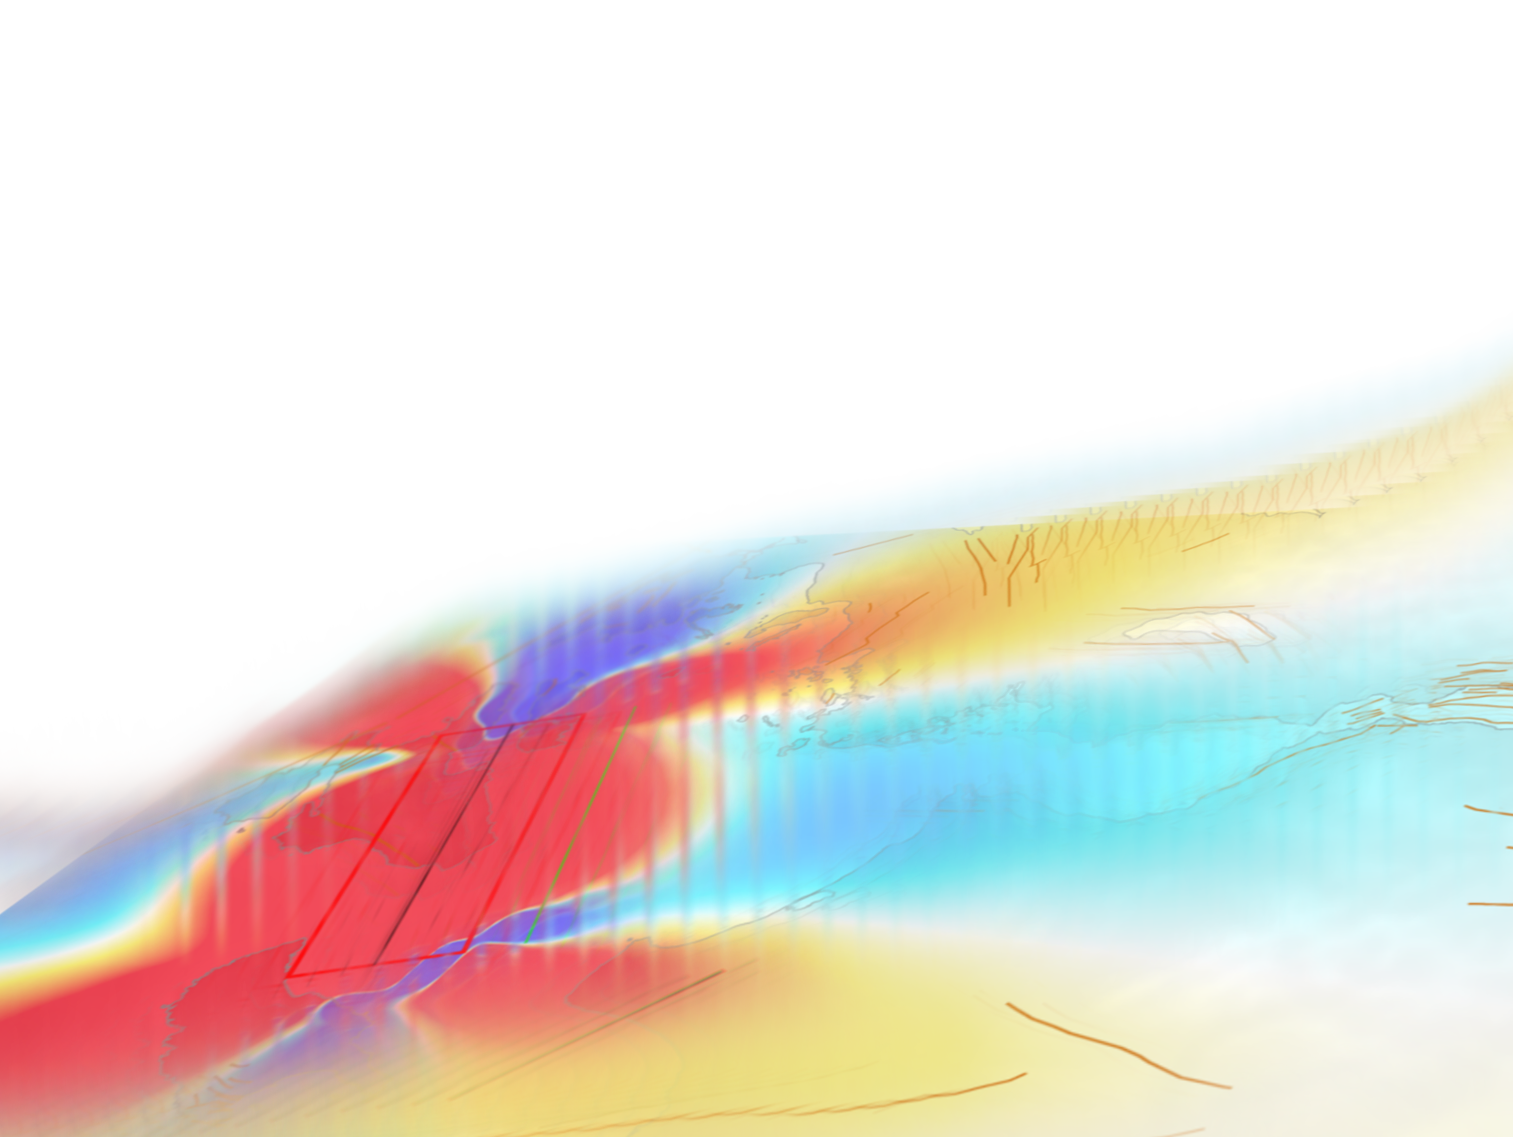
\includegraphics[width=.64\linewidth]{kef_1953_kef.png}
  \end{column}
  \begin{column}{.5\textwidth}
  \begin{scriptsize}
\begin{verbatim}
$ ./coulomb2gmt.sh kef_1953 kef_1953_kef \
                   -outjpg -o example401 \
                   -r 20.1 20.2 31.2 35.2 1000000
\end{verbatim}
\end{scriptsize}
\centering
  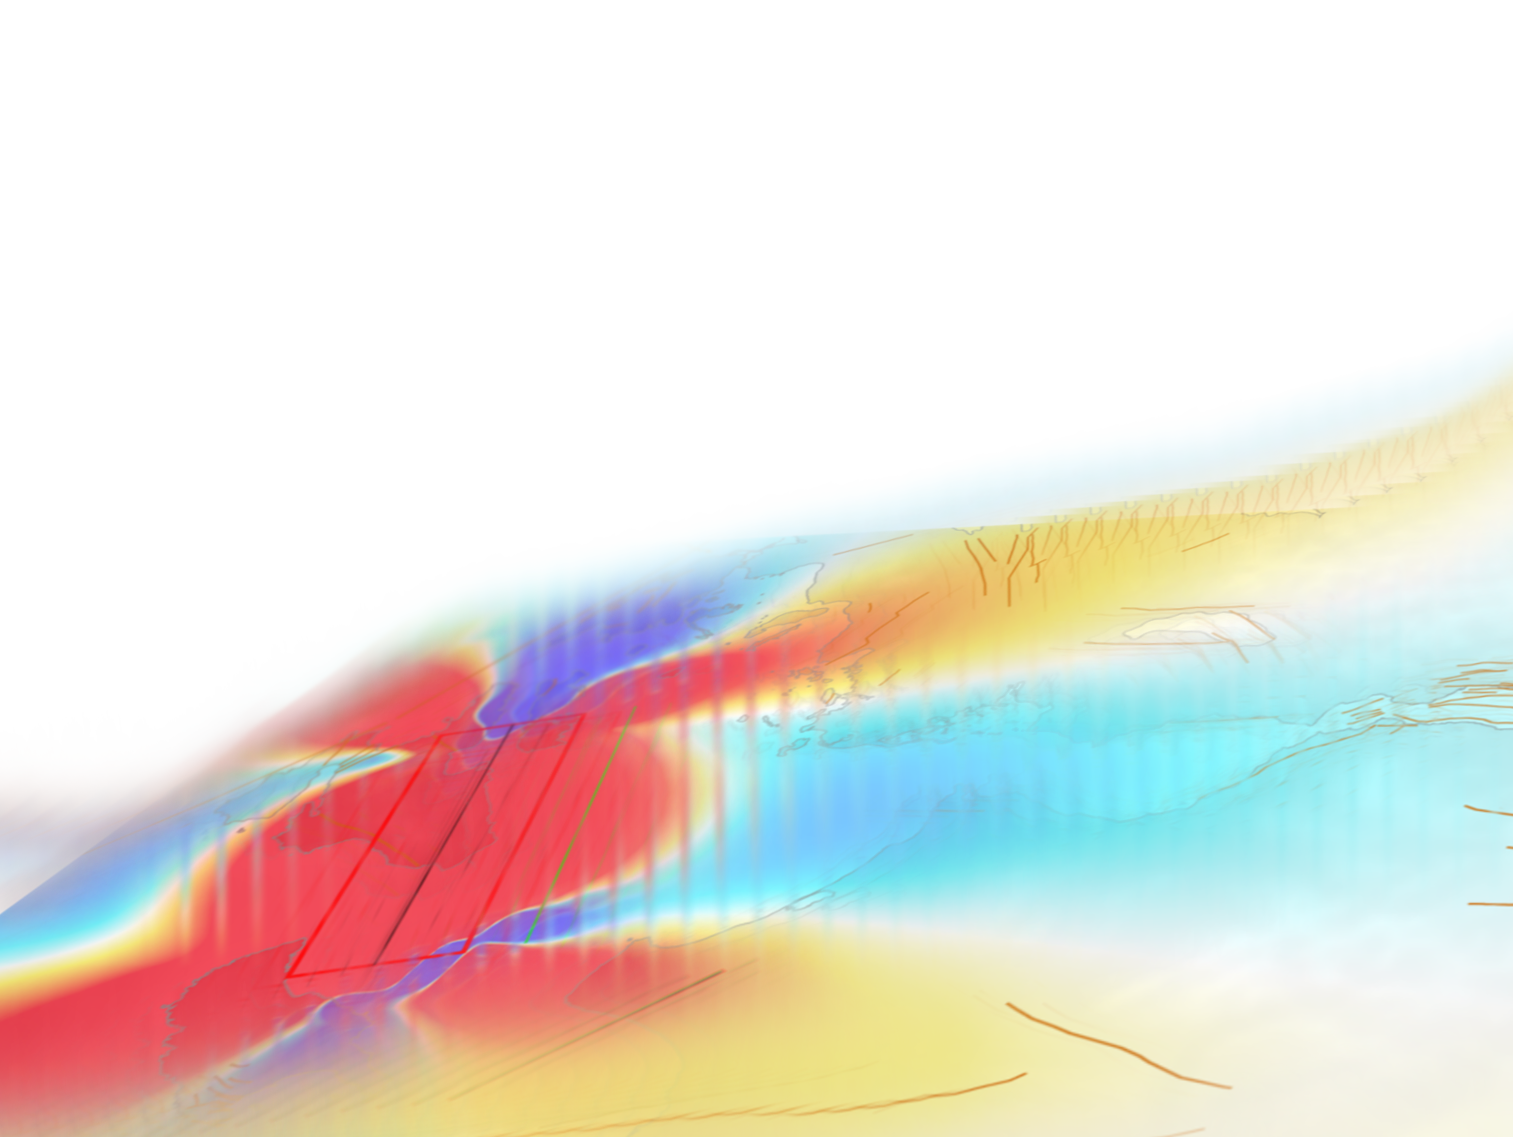
\includegraphics[width=.64\linewidth]{kef_1953_kef.png}
  \end{column}
\end{columns}

\end{frame}
\note{}

% //////////////////////////////////////////////////////////////////////////////
\begin{frame}[t,fragile]
  \frametitle{General Options - source faults}
  \framesubtitle{Plot fault parameters}
  \label{fr4:hist_pics}
\begin{columns}[t]
  \begin{column}{.5\textwidth}
\begin{scriptsize}
\begin{verbatim}
$ ./coulomb2gmt.sh kef_1953 kef_1953_kef \
                   -outjpg -o example401 \
\end{verbatim}
\end{scriptsize}
\centering
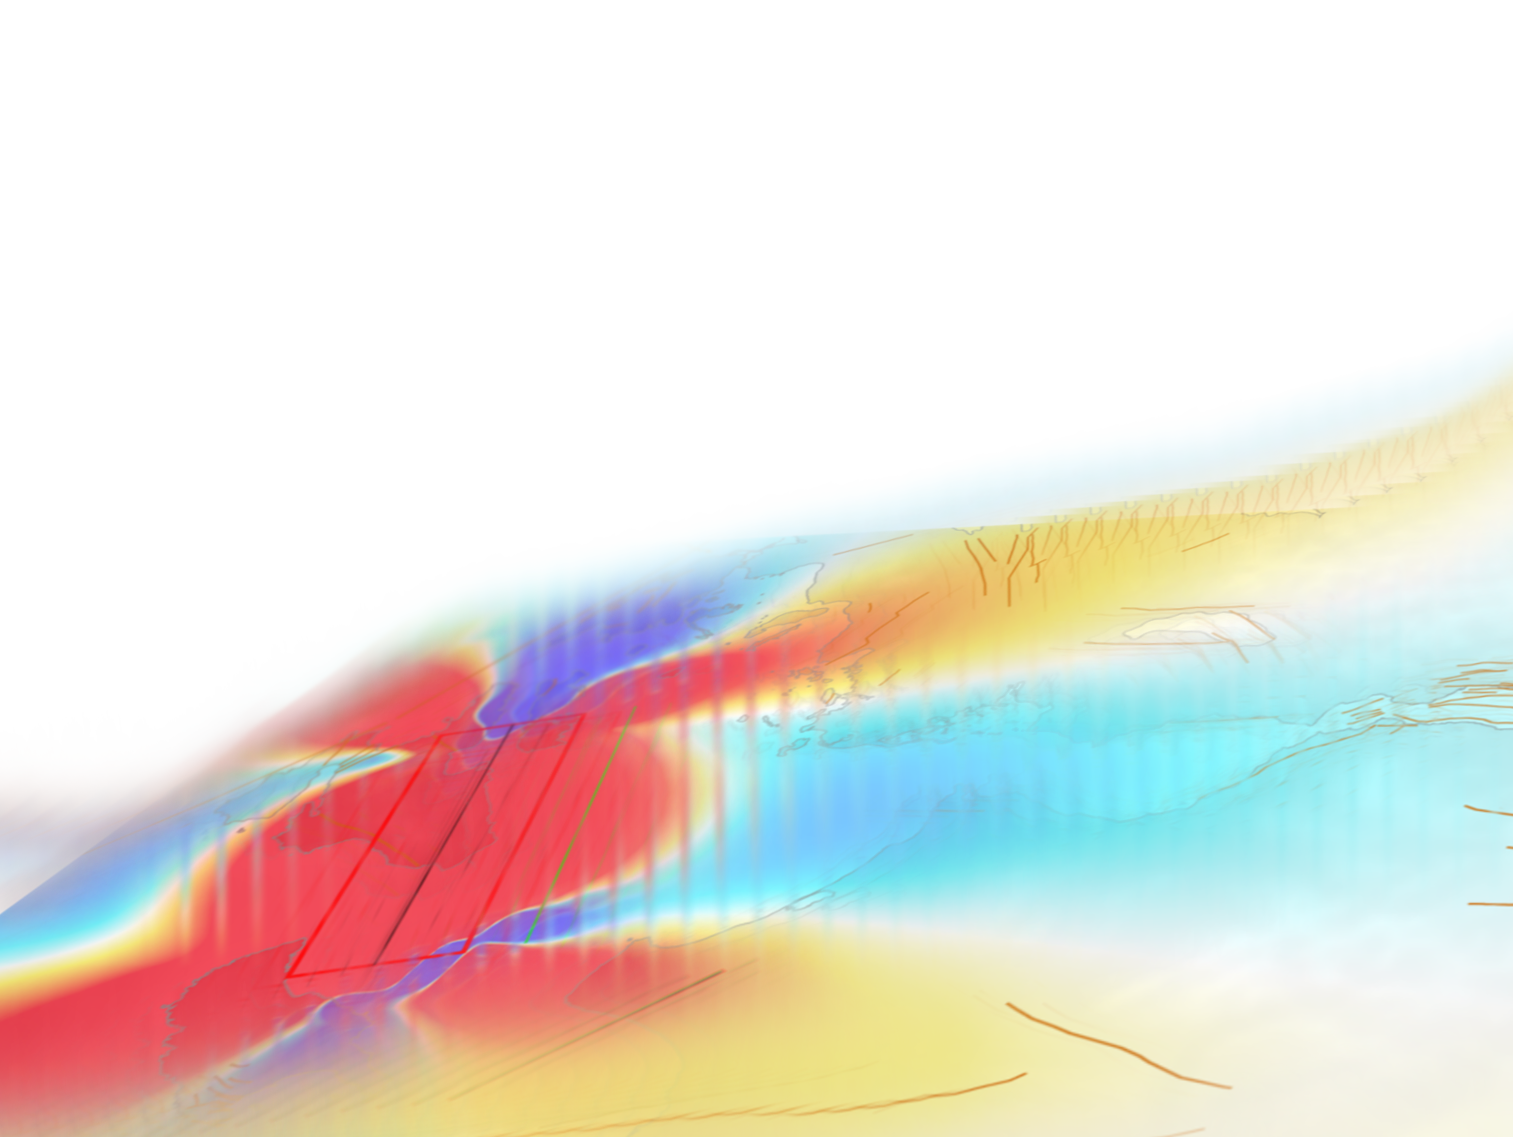
\includegraphics[width=.64\linewidth]{kef_1953_kef.png}
  \end{column}
  \begin{column}{.5\textwidth}
  \begin{scriptsize}
\begin{verbatim}
$ ./coulomb2gmt.sh kef_1953 kef_1953_kef \
                   -outjpg -o example402 \
                   -r 20.1 20.2 31.2 35.2 1000000
\end{verbatim}
\end{scriptsize}
\centering
  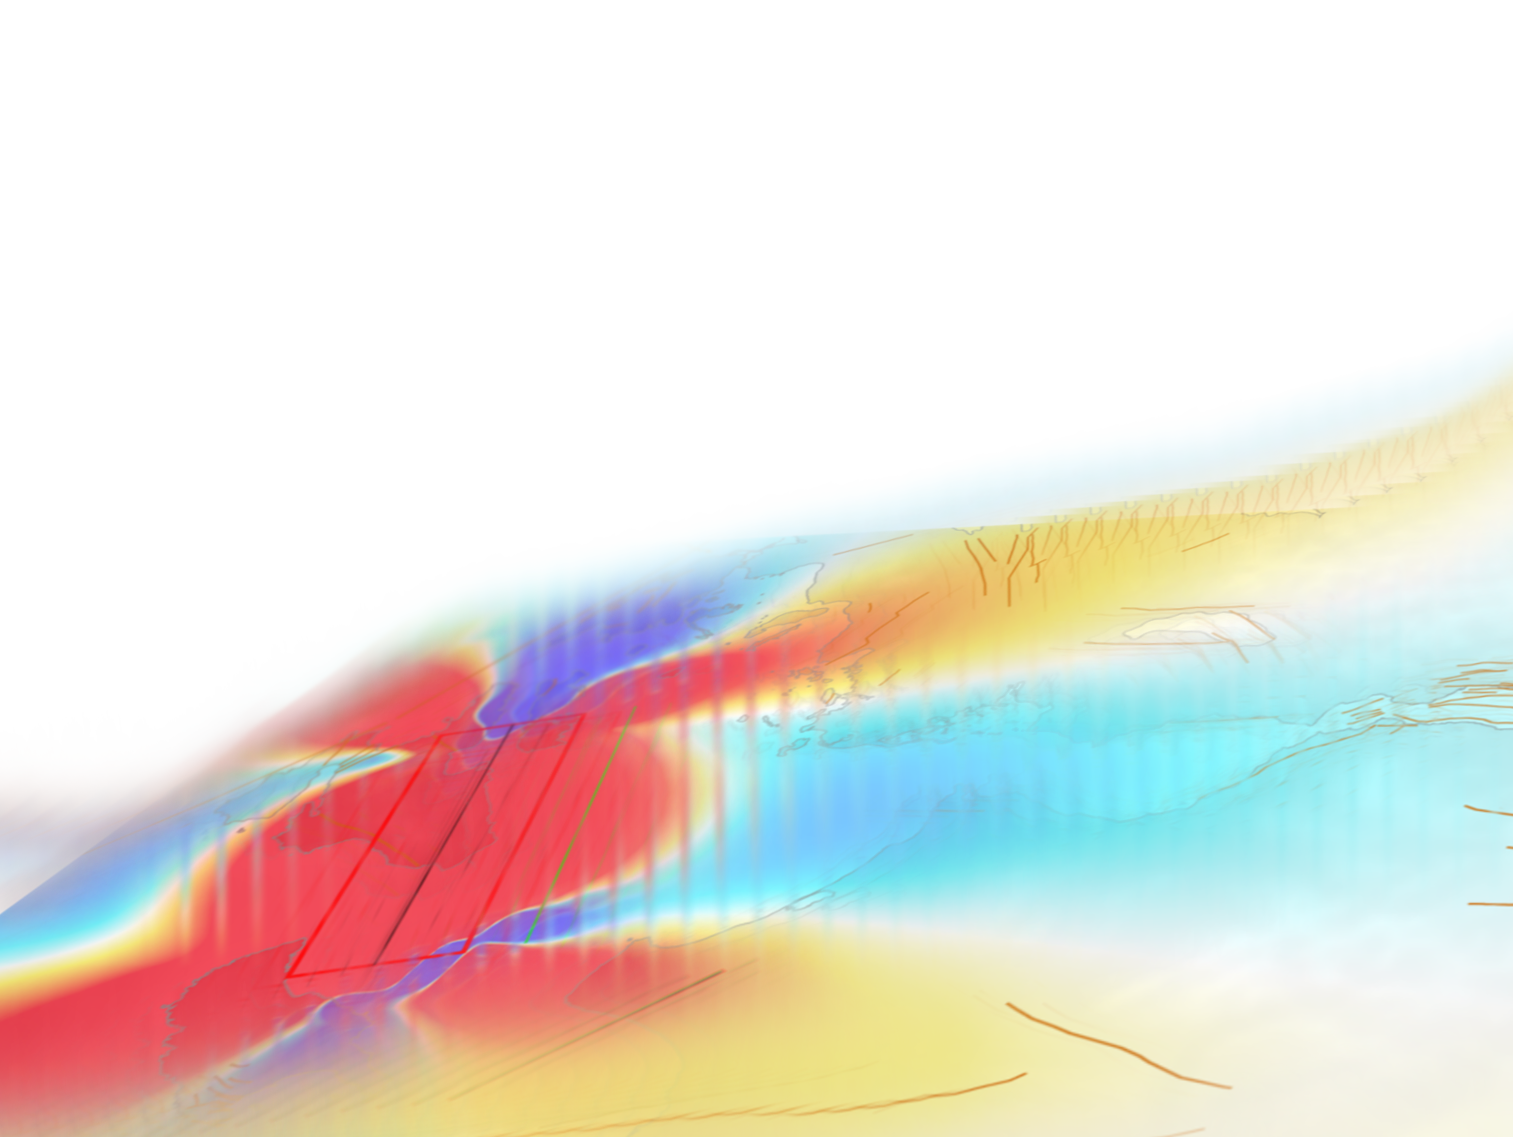
\includegraphics[width=.64\linewidth]{kef_1953_kef.png}
  \end{column}
\end{columns}

\end{frame}
\note{}

% //////////////////////////////////////////////////////////////////////////////
\begin{frame}[t,fragile]
  \frametitle{General Options - source faults}
  \framesubtitle{Plot fault parameters}
  \label{fr4:hist_pics}
\begin{columns}[t]
  \begin{column}{.5\textwidth}
\begin{scriptsize}
\begin{verbatim}
$ ./coulomb2gmt.sh kef_1953 kef_1953_kef \
                   -outjpg -o example403 \
                   -t
\end{verbatim}
\end{scriptsize}
\centering
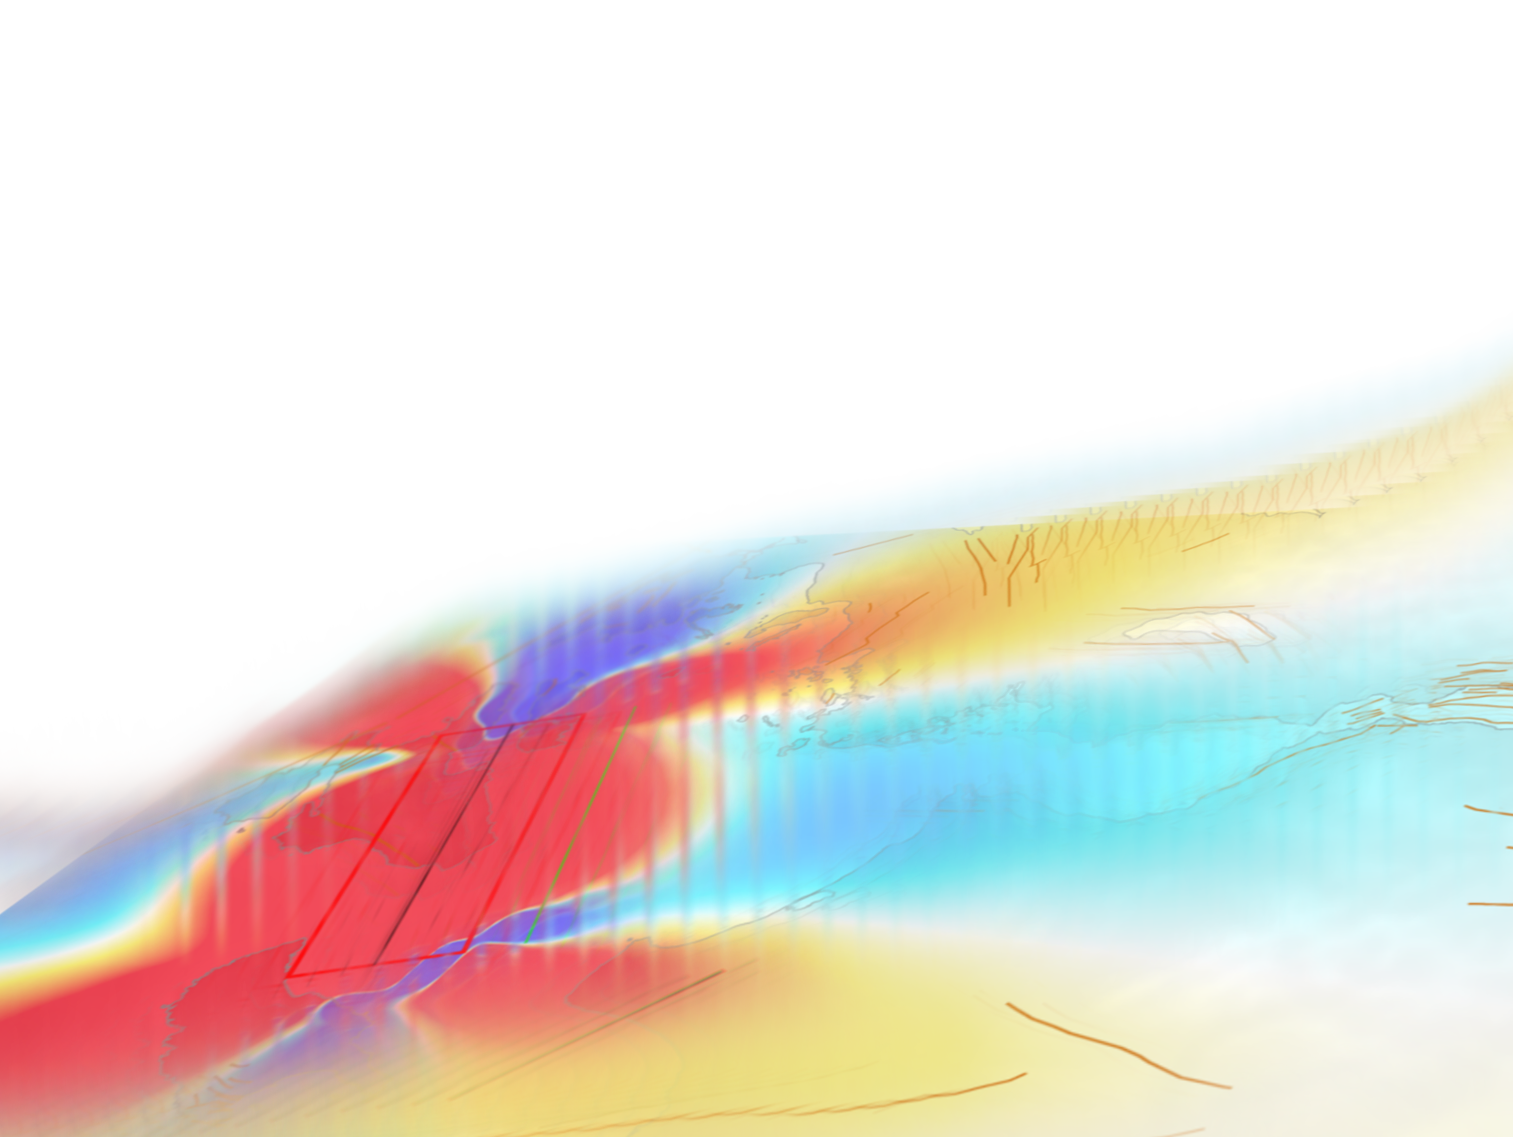
\includegraphics[width=.64\linewidth]{kef_1953_kef.png}
  \end{column}
  \begin{column}{.5\textwidth}
  \begin{scriptsize}
\begin{verbatim}
$ ./coulomb2gmt.sh kef_1953 kef_1953_kef \
                   -outjpg -o example404 \
                   -t -lg -lc
\end{verbatim}
\end{scriptsize}
\centering
  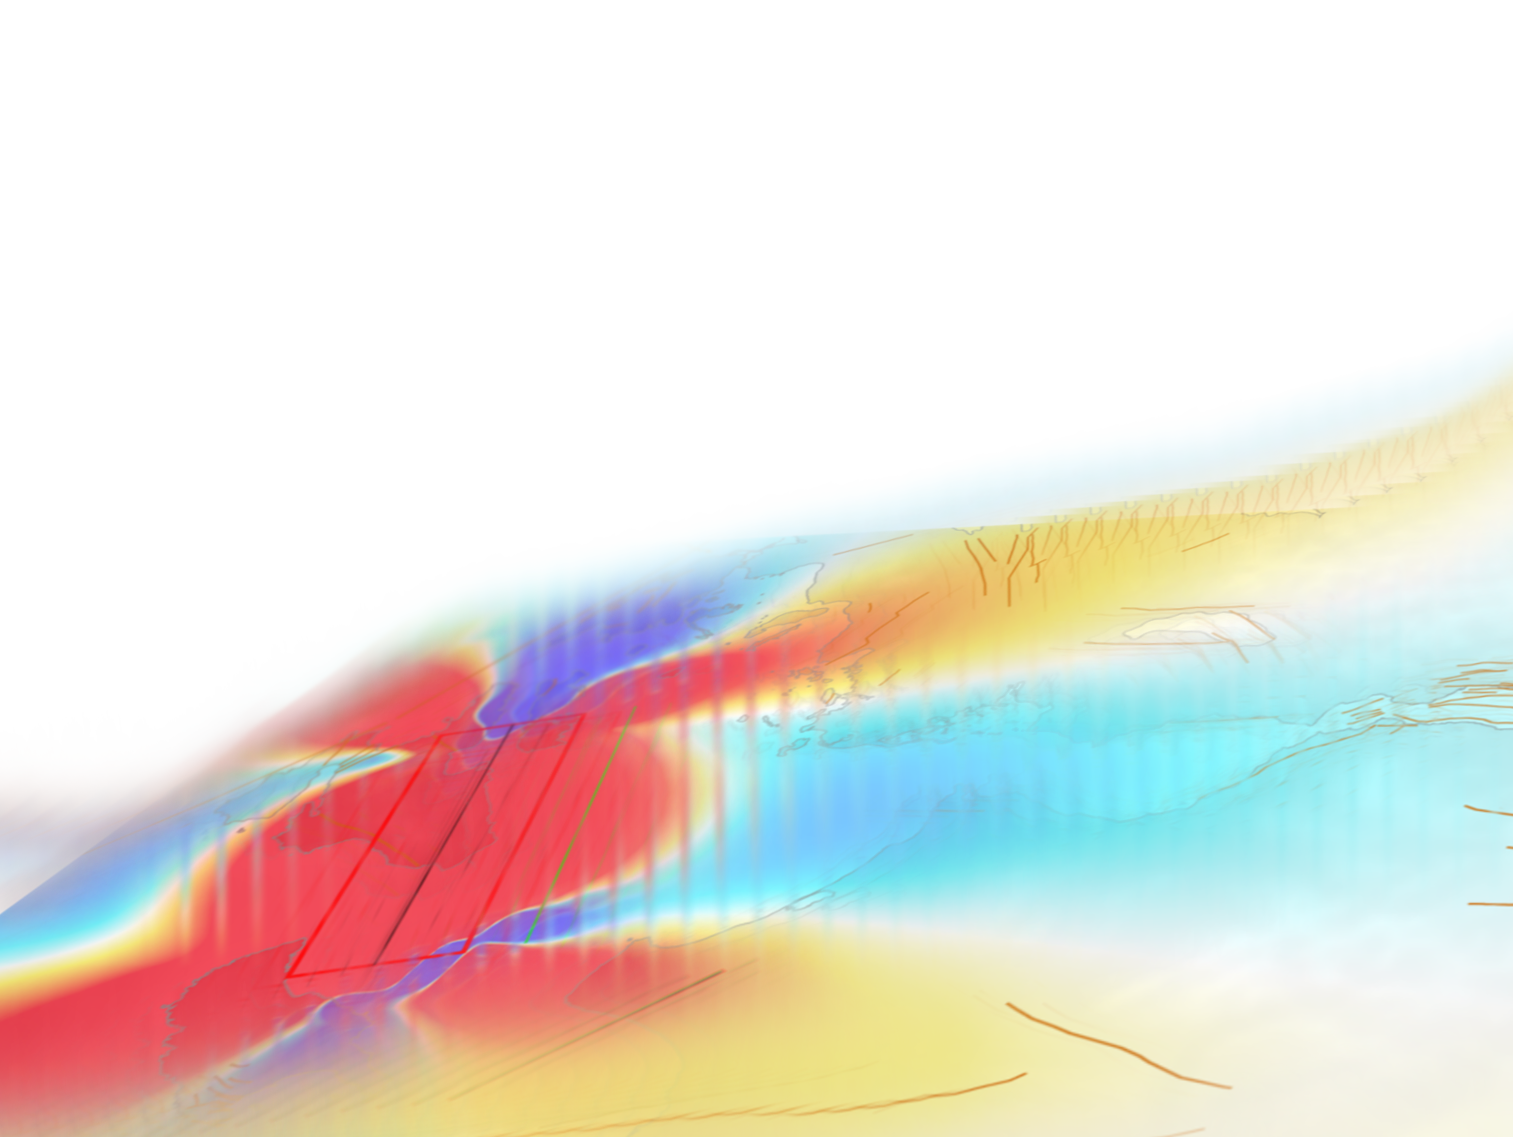
\includegraphics[width=.64\linewidth]{kef_1953_kef.png}
  \end{column}
\end{columns}

\end{frame}
\note{}

% //////////////////////////////////////////////////////////////////////////////
\begin{frame}[t,fragile]
  \frametitle{General Options - source faults}
  \framesubtitle{Plot fault parameters}
  \label{fr4:hist_pics}
\begin{columns}[t]
  \begin{column}{.5\textwidth}
\begin{scriptsize}
\begin{verbatim}
$ ./coulomb2gmt.sh kef_1953 kef_1953_kef \
                   -outjpg -o example405 \
                   -t -lg -lc \
                   -fproj -fsurf -fdep
\end{verbatim}
\end{scriptsize}
\centering
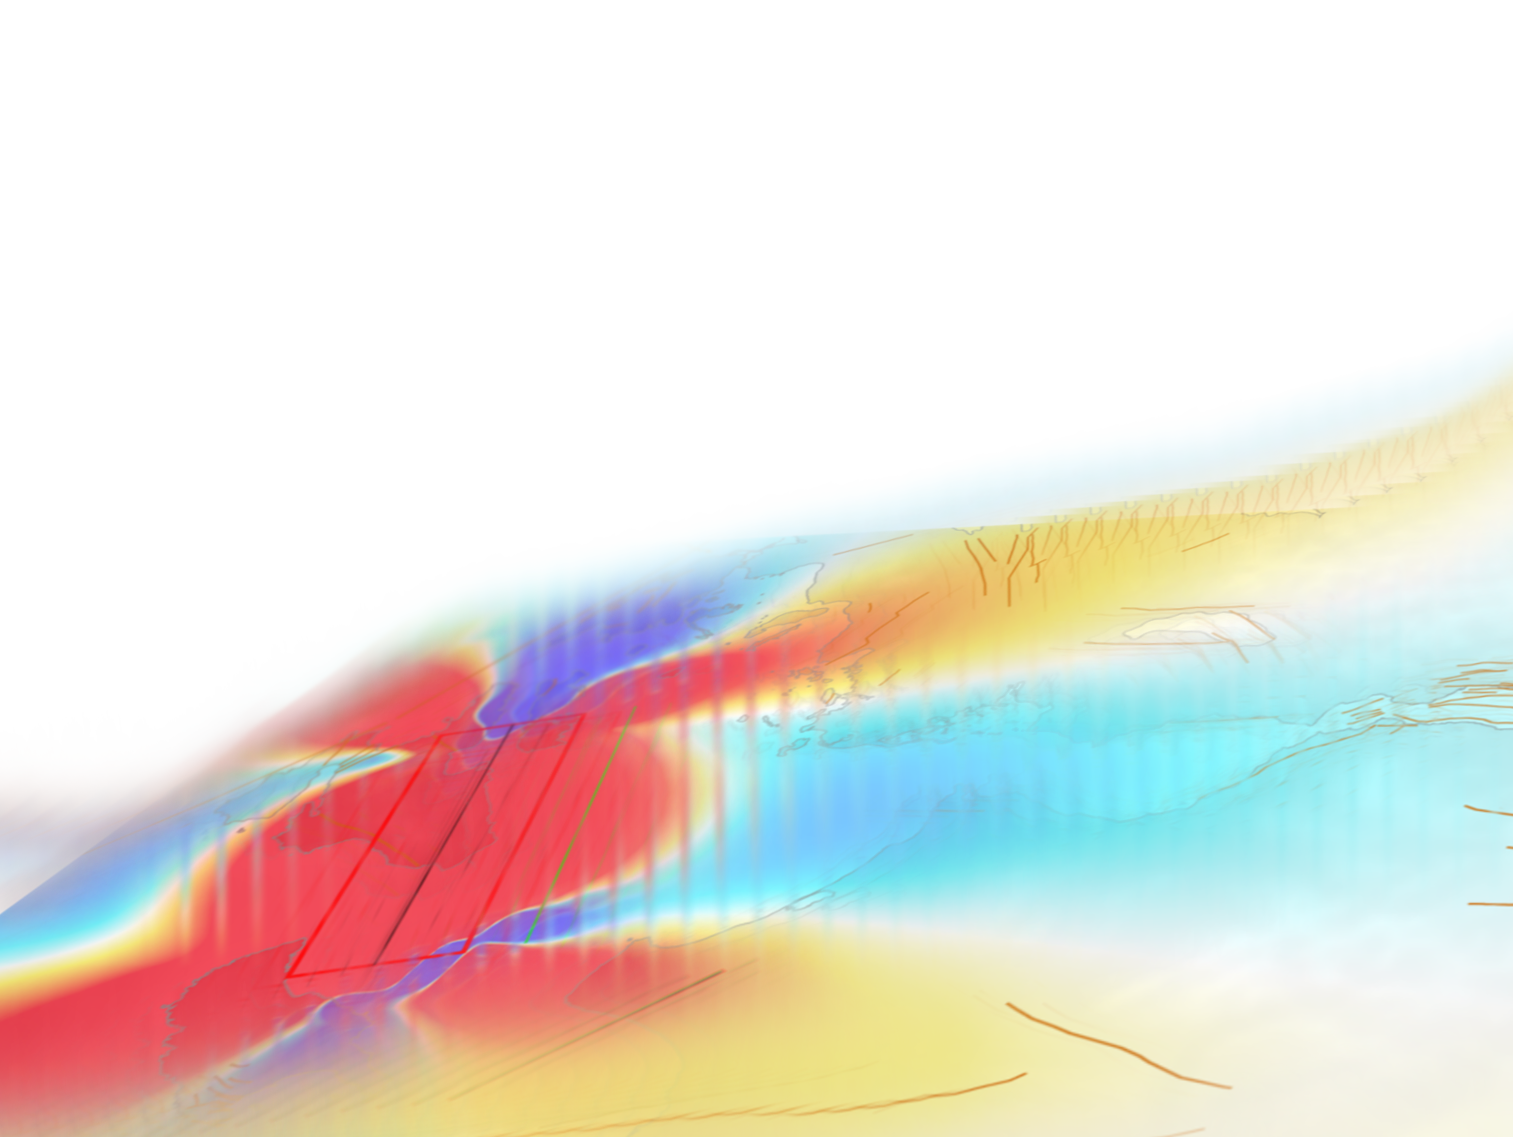
\includegraphics[width=.64\linewidth]{kef_1953_kef.png}
  \end{column}
  \begin{column}{.5\textwidth}
  \begin{scriptsize}
\begin{verbatim}
$ ./coulomb2gmt.sh kef_1953 kef_1953_kef \
                   -outjpg -o example406 \
                   -t -lg -lc \
                   -fproj -fsurf -fdep \
                   -cmt historic.cmt
\end{verbatim}
\end{scriptsize}
\centering
  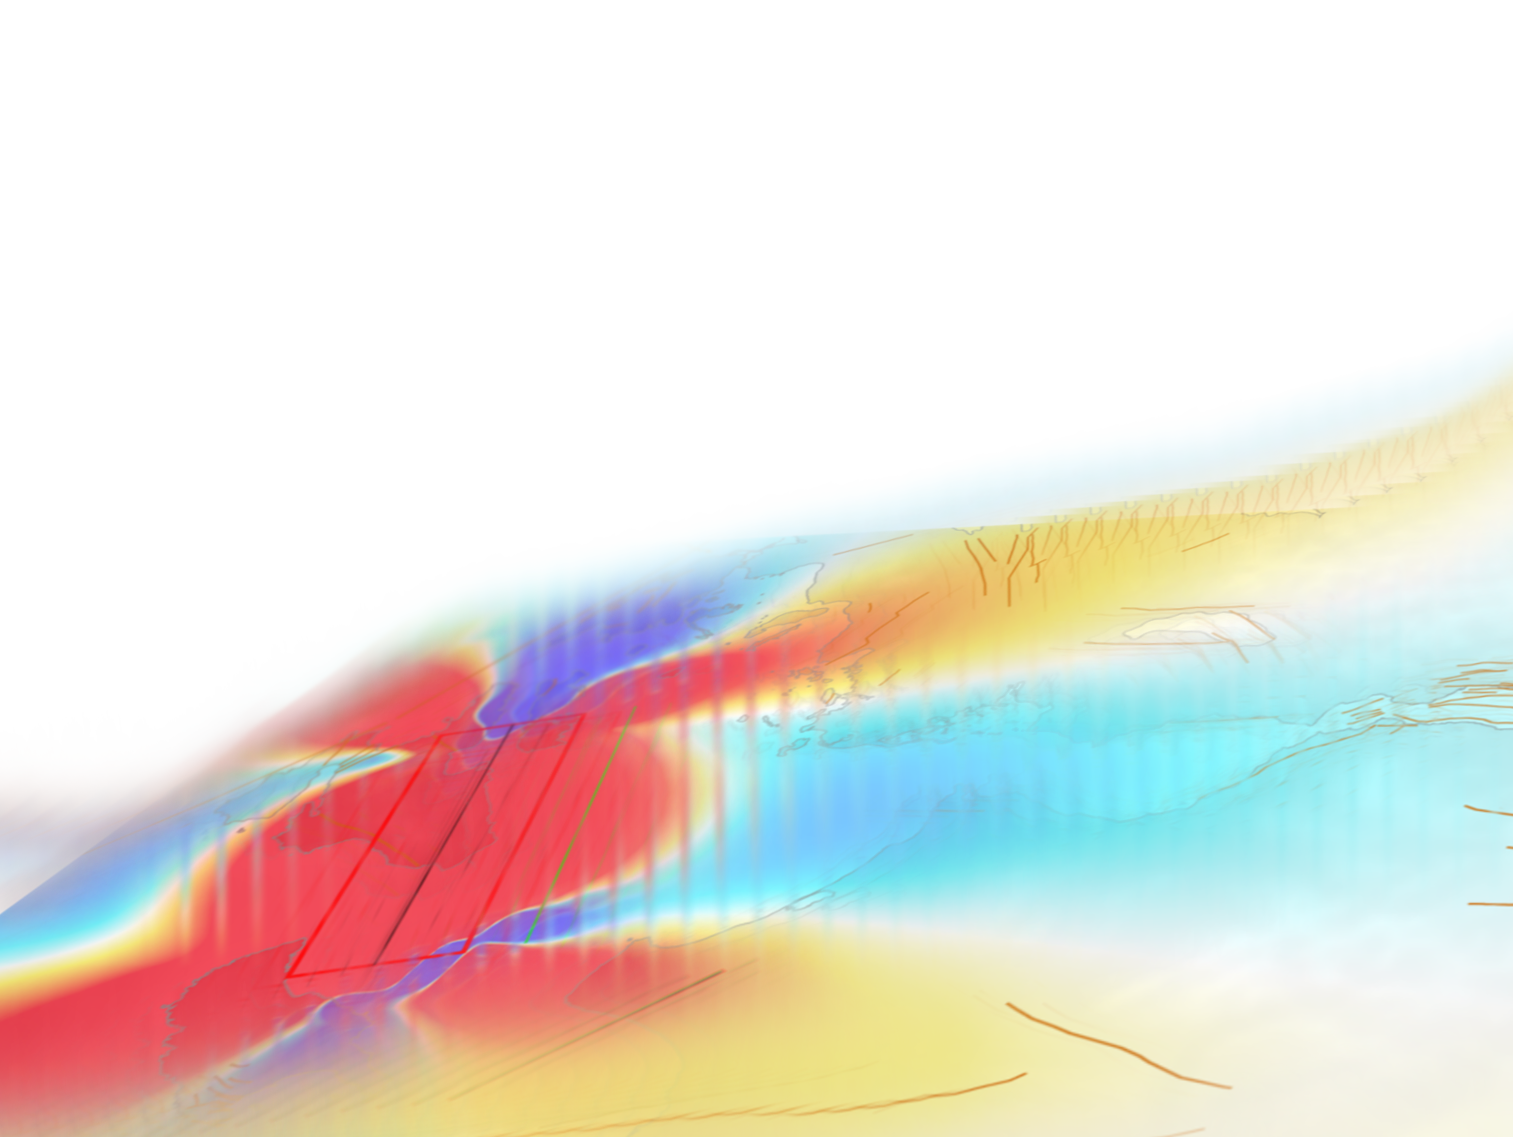
\includegraphics[width=.64\linewidth]{kef_1953_kef.png}
  \end{column}
\end{columns}

\end{frame}
\note{}

% //////////////////////////////////////////////////////////////////////////////
\begin{frame}[t,fragile]
  \frametitle{General Options - source faults}
  \framesubtitle{Plot fault parameters}
  \label{fr4:hist_pics}
\begin{columns}[t]
  \begin{column}{.5\textwidth}
\begin{scriptsize}
\begin{verbatim}
$ ./coulomb2gmt.sh kef_1953 kef_1953_kef \
                   -outjpg \ 
                   --output example407 \
                   --topography \
                   --logo_gmt \
                   --logo_custom \
                   --moment_tensor historic.cmt \
                   --eq_distribution CAT2014.TXT \
                   --map_title "Example 407" \
                   -fproj \
                   -fsurf \
                   -fdep
\end{verbatim}
\end{scriptsize}

  \end{column}
  \begin{column}{.5\textwidth}

\centering
  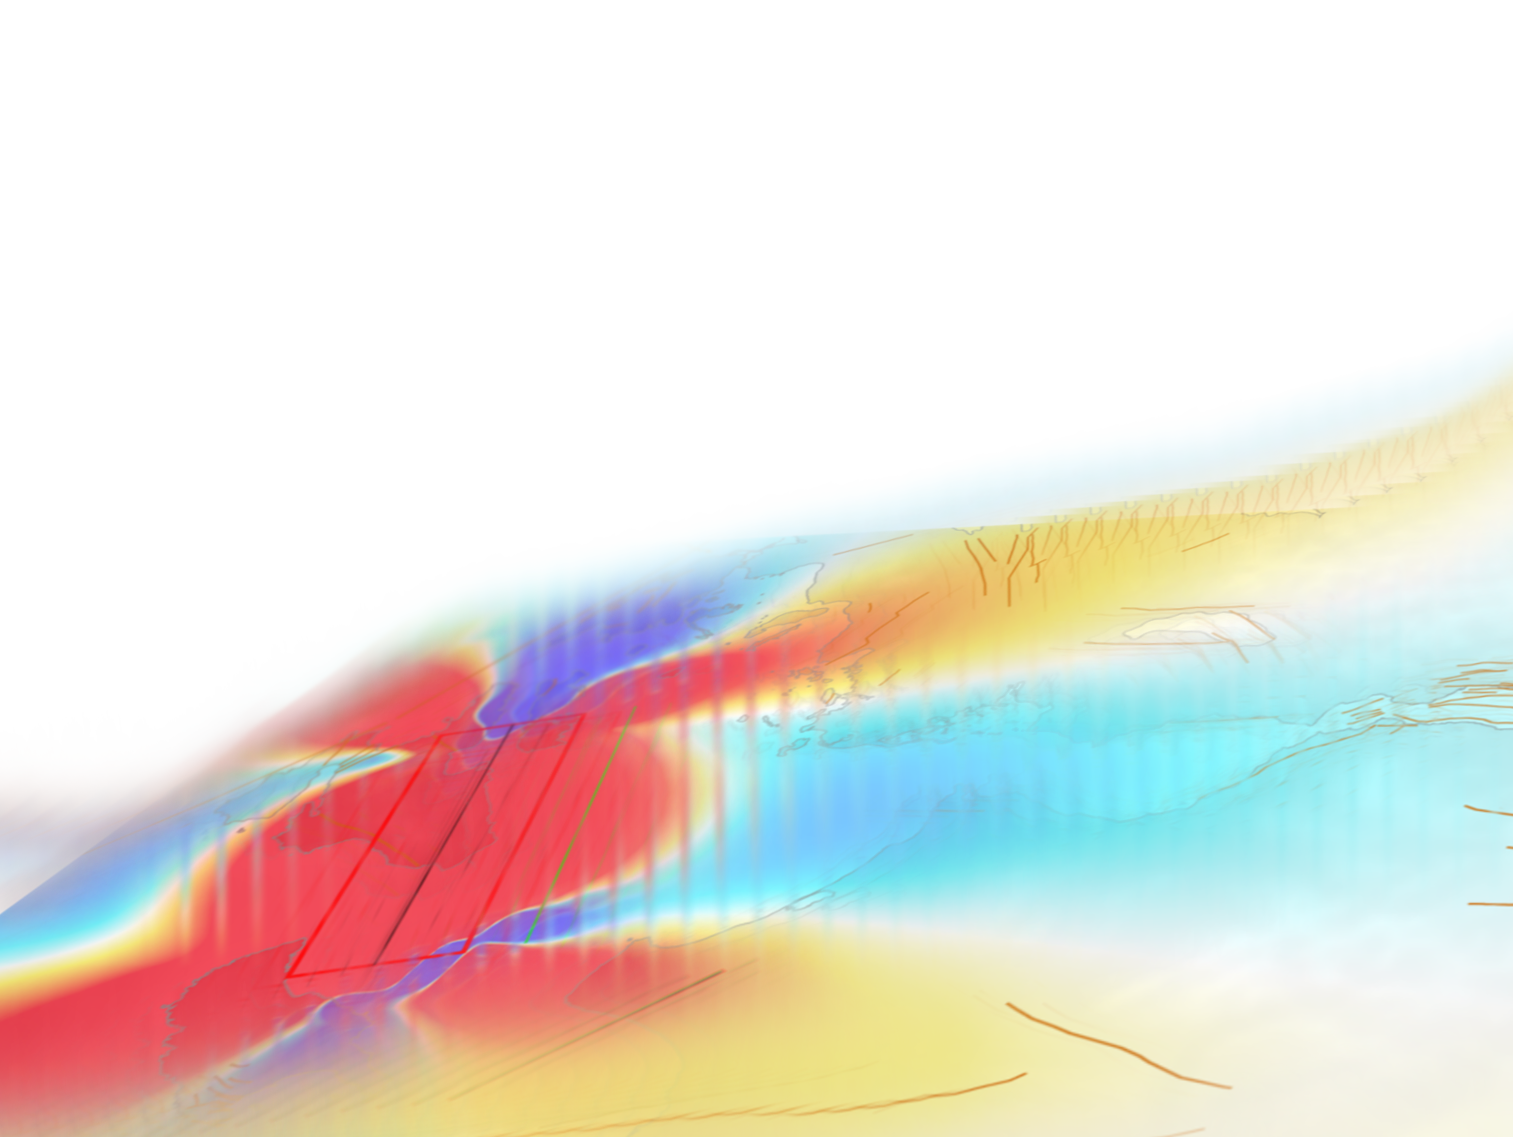
\includegraphics[width=.64\linewidth]{kef_1953_kef.png}
  \end{column}
\end{columns}

\end{frame}
\note{}

























